\chapter{Observations using the PyCBC modeled search pipeline}


In this chapter, I will discuss the PyCBC modeled search pipeline which is primarily designed for detecting and analyzing signals from merging binary systems of compact objects like black holes and neutron stars. It is one of the three major search pipelines that are used to create catalogs of binary merger observations. Since the inception, this pipeline has detected $\sim$ 100 binary mergers. The PyCBC pipeline is highly modular, allowing researchers to adapt its components for different types of analyses. This includes the ability to search for different types of gravitational wave sources, handle various noise artifacts in the detector data, and perform statistical analyses to assess the significance of potential detections.

We will also discuss the gravitational wave catalogs produced using this pipeline as an independent analysis to the LVK results: these were the third (3OGC) and the fourth (4OGC) open gravitational wave catalogs. 

PyCBC is an open-source software package, which allows for collaborative development and improvement by the scientific community. This openness not only fosters transparency in the data analysis methods used in gravitational wave astronomy but also encourages the adoption and adaptation of these techniques in other fields of physics and astronomy.

\section{Description of the PyCBC search pipeline}

\subsubsection{Inputs to the search pipeline}
There are two major inputs to the search pipeline -- 1) GW strain data from one or more detectors and 2) bank of templates corresponding to binary systems that we are searching for. We begin with strain data from the GW observatories typically sampled at a uniform sampling rate of 4098 Hz. This data contains glitches or noise artefacts based on the information provided by a specific auxillary channel. The quality of a data segment is characterized by a data quality flag. Some of the relevant flags are described below:
\begin{enumerate}
    \item DATA: Indicates unavailability of LIGO or Virgo data.
    \item CAT1: Signifies a critical issue with a detector component, leading to major known problems. CAT1 failures are consistent across data analysis groups and such data is not openly accessible.
    \item CAT2: Represents known physical interferences, like high seismic activity, affecting the gravitational wave channel.
    \item CAT3: Indicates unexplained statistical interferences in the gravitational wave channel.
\end{enumerate}

Data-quality investigations might fail to remove all the noise transients. Usually short duration loud transients of order of 1s having SNR $\sim (100--1000)$ can creep in the data. These transients can severely affect the sensitivity of the search by creating large number of spurious triggers. A procedure called \textit{gating} is used to mask the corrupted data around the glitch and to reduce the noise background by removing the spurious noise triggers. 

The second input to the search is the template bank. As described in [], the template bank consists of discrete sets of points over the intrinsic parameters of GW sources. A search for aligned-spin quasi-circular systems typically uses four parameters in a template bank -- detector frame component masses $m_{1}^{det}, m_{2}^{det}$ and component spins $s_{1z}, s_{2z}$. In case of searches for eccentric or precessing sources, additional parameters needs to be incorporated. 

The creation of a template bank entails strategically choosing discrete points within the parameter space. This ensures that any point within the permissible region is within a maximum distance, $ d_{\text{max}} $, from a sampled point. This distance is defined by the mismatch in waveform at these points. The mismatch level dictates the template bank's density and requires careful calibration. A higher mismatch value results in fewer templates, potentially reducing signal SNR, while a lower value increases the number of templates, raising computational demands for matched filtering. The challenge lies in optimizing the number of templates while preserving a set minimum match (1 - mismatch). Various techniques for generating a template bank fall into three main categories: geometric lattice-based methods, stochastic placement algorithms, and hybrid approaches.

Sampling the parameter space by computing mismatches between different waveforms require estimation of noise PSD from the data. A single PSD is used that is valid for the entire search duration to create a single template bank for a detector network. The procedure begins by separately estimating PSDs for each detector in the network using the Welch's method. Data segments of 512s is subdivided into several 16s blocks to estimate PSDs in each block -- for each segment 63 PSDs are estimated. Then the median of the several 16s PSDs is computed to average the power spectrum for the corresponding data segment. Noise PSDs from each segments are combined together as a harmonic mean for the given detector. Repeating the previous steps for each detector and finally taking the average PSD over all detector gives the PSD that is used in generating the template bank. 


\subsubsection{Matched Filtering}
At its core, the PyCBC search pipeline employs the matched-filtering technique. The inputs to the pipeline are discrete quantities -- data $s[t_i]$, templates $h[t_i; \zeta]$ described by parameters $\zeta$, and noise PSD $S_n[f_i]$. The data and the templates are transformed to their Fourier-domain equivalents $\tilde{s}[f_i]$ and $\tilde{h}[f_i]$ respectively, using the Fast Fourier Transform (FFT) algorithm in blocks of $T_B = 512$s. The average PSD is estimated for each block using the median method as discussed previously. Computation of FFTWs is implemented via Intel's Math Kernel Libray on computer processing units (CPUs) or via Nvidia's CUDA library on graphical processing units (GPUs), these libraries are efficient in performing FFTWs in several batches in parallel.  


The discrete form of the Fourier-domain matched filtering equation is given by

\begin{align}
    \rho^2[t_j] \equiv \innerprod{s}{h[\zeta]}[t_j] = 4 \Delta f \sum_{k=1}^{(N-1)/2} \dfrac{\tilde{s}[k]\tilde{h}^*[k;\zeta]}{S_n[k]}e^{2i\pi j k/N},
\end{align}

giving us the matched-filter SNR time series $\rho^2[t_j]$ for a template with the parameters $\zeta$. When the SNR is above a fixed threshold (usually $\sim 5$) then a \textit{trigger} is associated to the corresponding timestamp and the triggering template. In each blocks, triggers are clustered in windows of 1s and only the loudest trigger is stored for further follow-up.  

\subsubsection{Signal Consistency Tests}
Add some intro


\textit{1. Mitigating noise artefacts}\\
Data quality checks and gating vetoes remove only the very loud non-Gaussian noise artefacts. Many glitches are still present in the data that contribute to long tails of the SNR distribution which reduces the significance of a real astrophysical event. The chi-squared test is used to distinguish noise triggers from signal triggers which typically requires intensive computation. It demands an extra $p-$ FFT operations for each SNR time series FFT calculation, corresponding to each frequency bin. The PyCBC pipeline, however, only computes the chi-squared test at clustered trigger times in the SNR series, using an optimized frequency integral rather than FFTs. This method is more efficient unless there's poor data quality with many triggers, where FFT is faster.  

\textit{2. Coincidence test}\\
To minimize the number of false alarms, the PyCBC pipeline also ensures that a potential event is detected with consistent parameters across all detectors. This involves a coincidence test on triggers after vetoing glitches. For a two-detector network, signals must be detected in both detectors within a 15 ms window, allowing for travel time and timing errors. Unlike previous searches that used a metric-based coincidence test, the PyCBC pipeline requires exact-match coincidence, meaning the triggers from each detector must have identical template parameters (masses and spins).

The exact-match test is especially useful for complex gravitational waveforms, like those from spinning neutron stars or black holes, or high-mass waveforms where stochastic templates are used. This method has shown a noticeable improvement in search sensitivity. Triggers passing this test are considered coincident events and are ranked based on a ranking statistic, which is discussed next.

\subsubsection{Ranking the candidates}


\begin{figure}
    \centering
    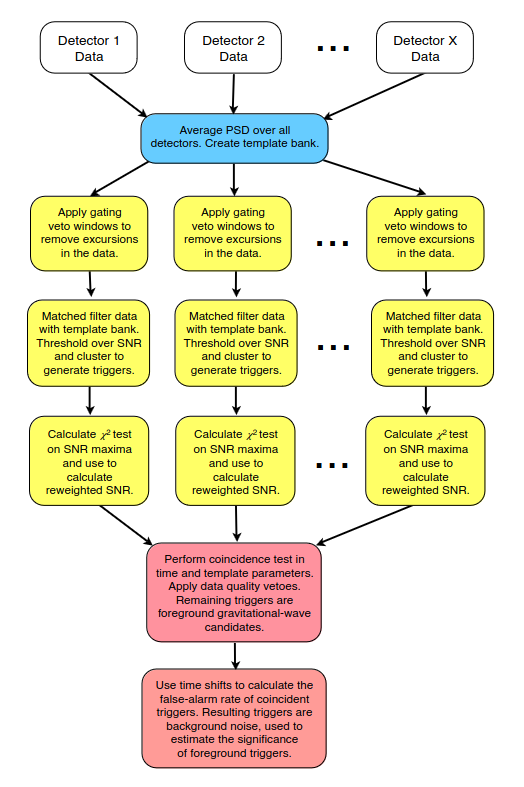
\includegraphics[width=0.75\linewidth]{search_workflow.png}
    \caption{Workflow of the PyCBC search pipeline}
    \label{fig:pycbc_search_workflow}
\end{figure}




\section{Sensitivity of a search}


\section{Current observations of gravitational wave events}
\subsection{The 4OGC and 3OGC catalogs}
\subsection{What do we know from current observations?  }


%Since the current advanced LIGO and advanced VIRGO detectors went online 